 
\chapter{Выбор рациональной конструкции}

В работе был проведен анализ весовых характеристик самолета для трех вариантов конструкции фюзеляжа. Варианты конструкции отличаются выбором силового короба, обеспечивающего надежное соединение задней части фюзеляжа с кессоном центроплана. 

%\section{Подбор оптимального размера конечного элемента}

Было построено 7 моделей с различным размером конечного элемента. Путем расчета моделей с заданными нагрузками были определены средние величины напряжений для стенок в наиболее напряженных отсеках (обозначены белым на  Рис.\ref{fig:WingRootPlain})

\begin{figure}[ht]
\centering
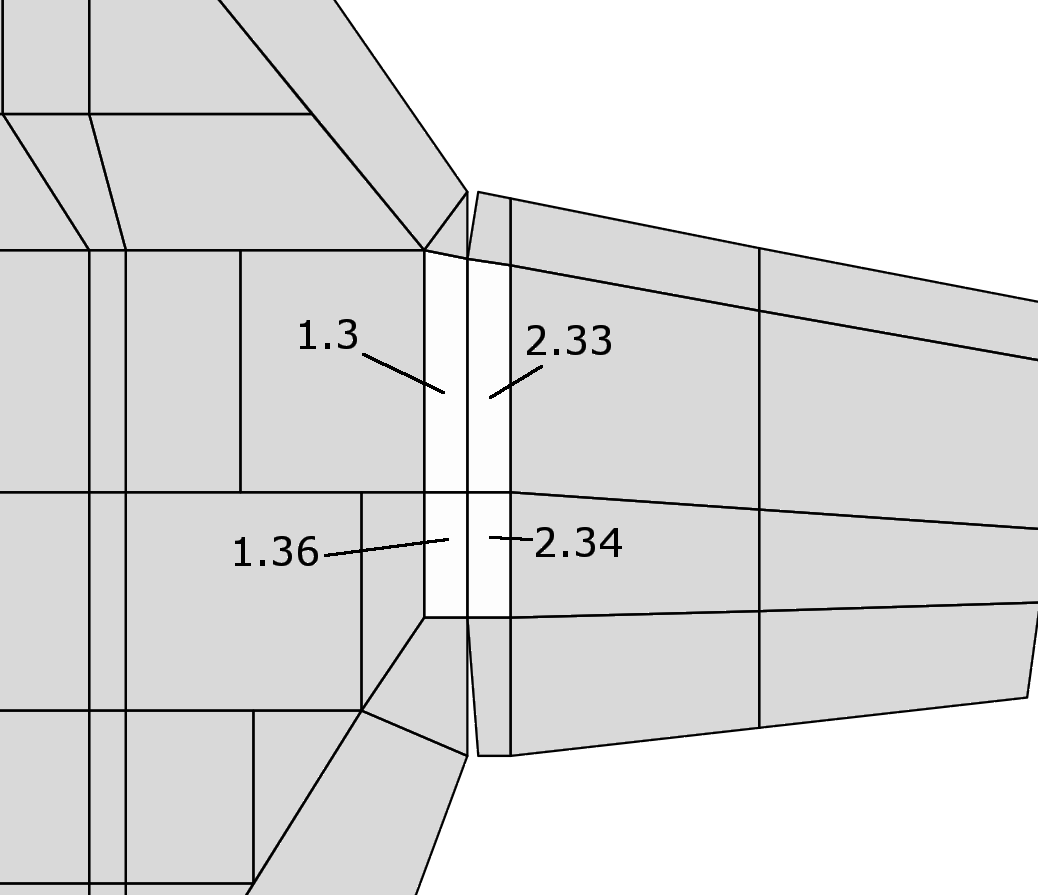
\includegraphics[width=0.6\textwidth]{RootOfWingWithSelectedPartsBW}
\caption{Стык правого крыла и фюзеляжа. Схематичное изображение вида сверху}
\label{fig:WingRootPlain}
\end{figure}


\begin{figure}[H]
\centering
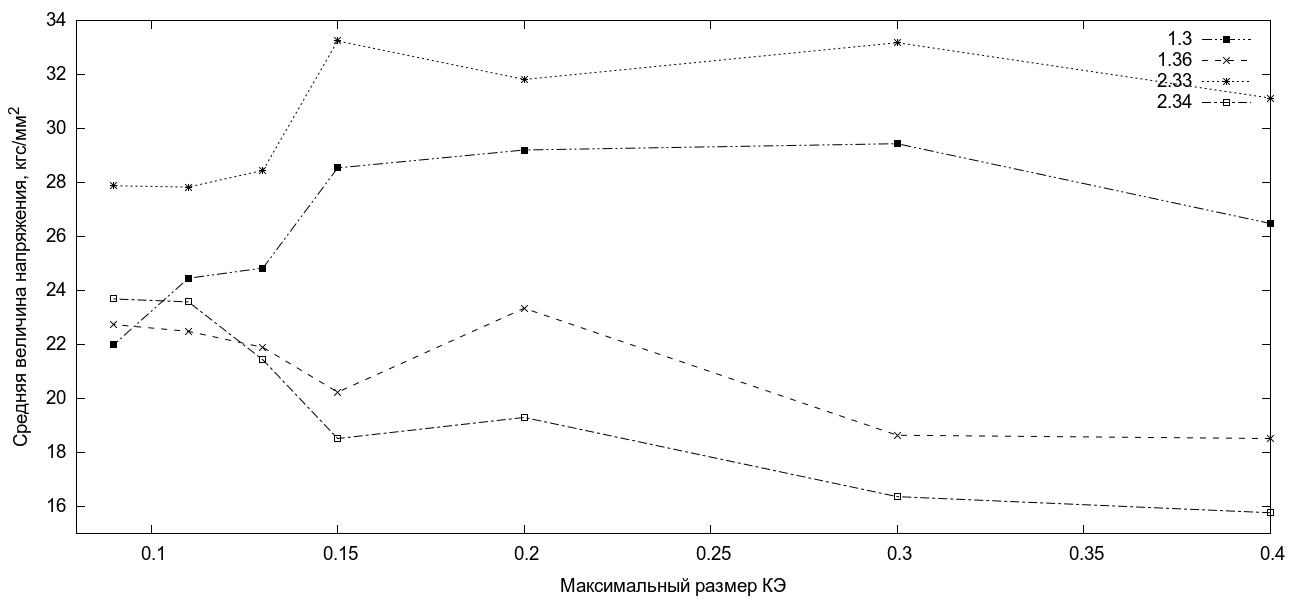
\includegraphics[width=0.8\textwidth]{StressToDiscretenessPlot}
\caption{Зависимость средних напряжений в отсеках от величины КЭ}
\label{fig:stressToDiscreteness}
\end{figure}

Была получена зависимость средних напряжений в этих отсеках от размера конечного элемента (Рис.\ref{fig:stressToDiscreteness})

На основании полученных данных была определена оптимальная величина конечного элемента для дальнейшей работы над моделью, равная $0,11\text{м}$. 
%Ниже приведены картины НДС в месте стыка крыла с фюзеляжем при различных размерах конечного элемента. 

\section{Подбор оптимальной дискретности модели}

В целях обеспечения точности расчета было проведено исследование зависимости напряженно-деформированного состояния самолета от максимального характерного размера конечных элементов, используемых в модели. 

С помощью программного комплекса ``Conver'' было построено 7 моделей самолета по одинаковой схеме с использованием различных размеров конечного элемента. Путем расчета моделей были определены средние величины напряжений для панелей и стенок в наиболее напряженных отсеках самолета (обозначены белым на  Рис.\ref{fig:WingRootPlain})

\begin{figure}[ht]
\centering
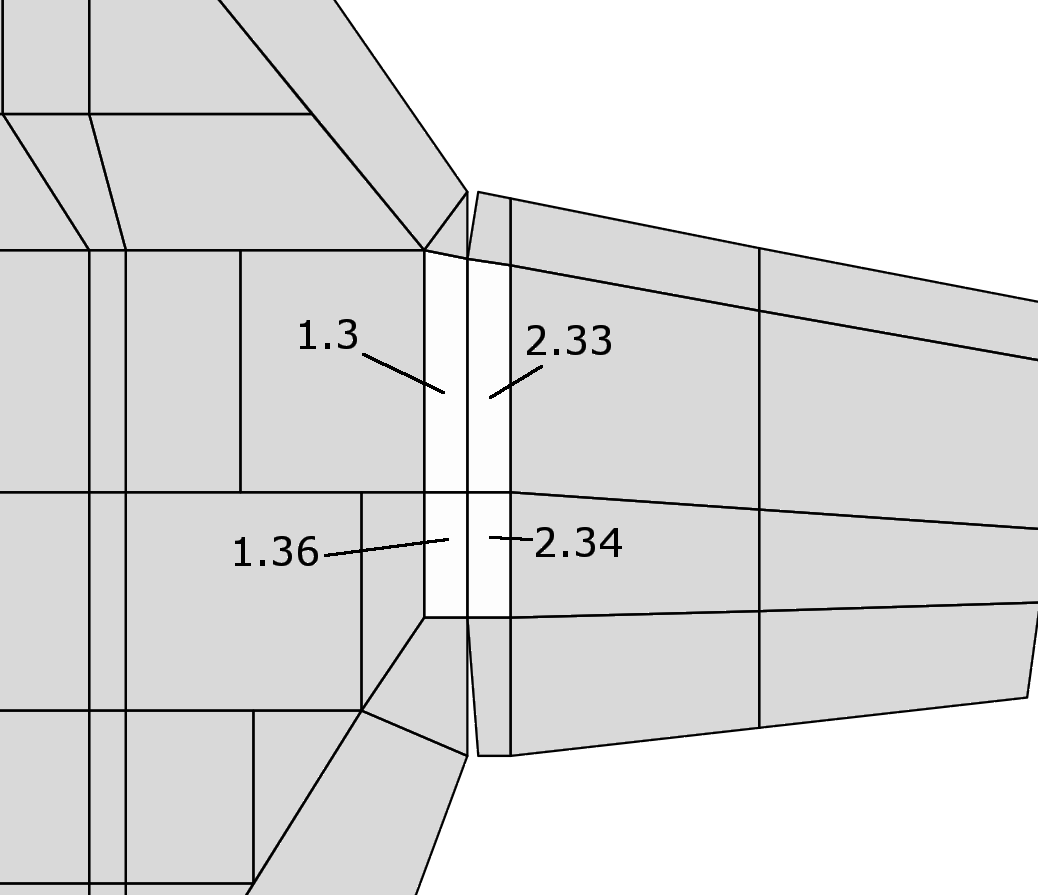
\includegraphics[width=0.5\textwidth]{RootOfWingWithSelectedPartsBW}
\caption{Схематичное изображение вида сверху в месте стыка правого крыла и фюзеляжа}
\label{fig:WingRootPlain}
\end{figure}




Исходя из полученных данных, была получена зависимость величины средних напряжений в панелях и стенках этих отсеков от выбора размера конечного элемента (Рис.\ref{fig:stressToDiscreteness})

\begin{figure}[H]
\centering
%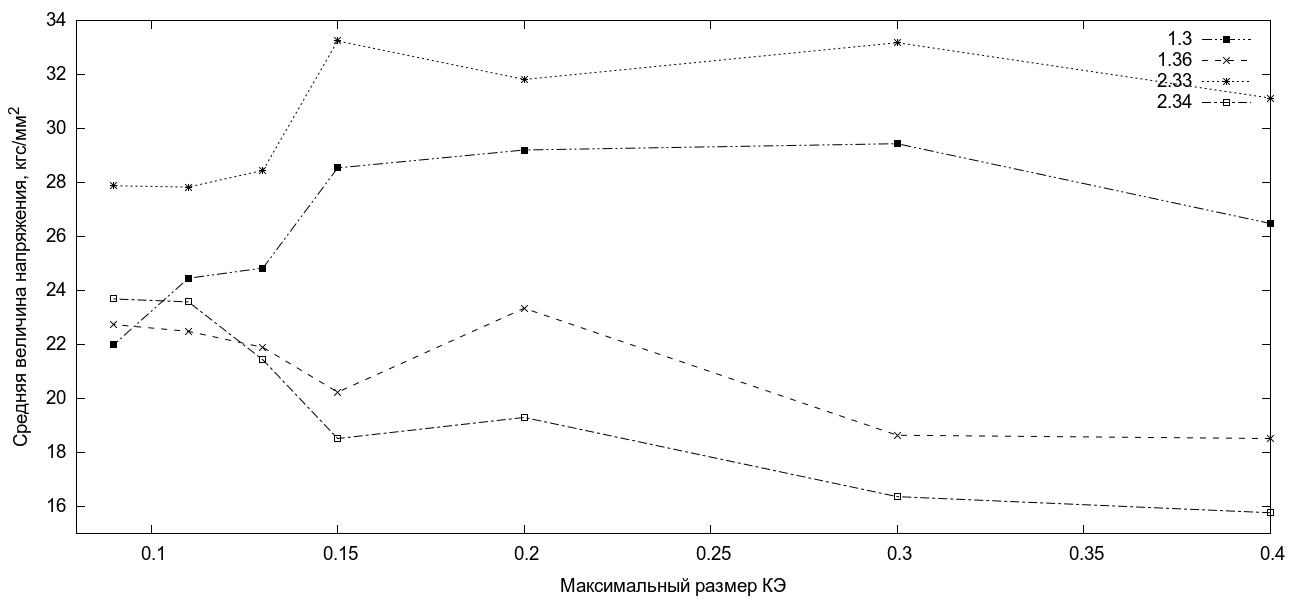
\includegraphics[width=0.8\textwidth]{StressToDiscretenessPlot}
% GNUPLOT: LaTeX picture with Postscript
\begingroup
  \makeatletter
  \providecommand\color[2][]{%
    \GenericError{(gnuplot) \space\space\space\@spaces}{%
      Package color not loaded in conjunction with
      terminal option `colourtext'%
    }{See the gnuplot documentation for explanation.%
    }{Either use 'blacktext' in gnuplot or load the package
      color.sty in LaTeX.}%
    \renewcommand\color[2][]{}%
  }%
  \providecommand\includegraphics[2][]{%
    \GenericError{(gnuplot) \space\space\space\@spaces}{%
      Package graphicx or graphics not loaded%
    }{See the gnuplot documentation for explanation.%
    }{The gnuplot epslatex terminal needs graphicx.sty or graphics.sty.}%
    \renewcommand\includegraphics[2][]{}%
  }%
  \providecommand\rotatebox[2]{#2}%
  \@ifundefined{ifGPcolor}{%
    \newif\ifGPcolor
    \GPcolorfalse
  }{}%
  \@ifundefined{ifGPblacktext}{%
    \newif\ifGPblacktext
    \GPblacktexttrue
  }{}%
  % define a \g@addto@macro without @ in the name:
  \let\gplgaddtomacro\g@addto@macro
  % define empty templates for all commands taking text:
  \gdef\gplbacktext{}%
  \gdef\gplfronttext{}%
  \makeatother
  \ifGPblacktext
    % no textcolor at all
    \def\colorrgb#1{}%
    \def\colorgray#1{}%
  \else
    % gray or color?
    \ifGPcolor
      \def\colorrgb#1{\color[rgb]{#1}}%
      \def\colorgray#1{\color[gray]{#1}}%
      \expandafter\def\csname LTw\endcsname{\color{white}}%
      \expandafter\def\csname LTb\endcsname{\color{black}}%
      \expandafter\def\csname LTa\endcsname{\color{black}}%
      \expandafter\def\csname LT0\endcsname{\color[rgb]{1,0,0}}%
      \expandafter\def\csname LT1\endcsname{\color[rgb]{0,1,0}}%
      \expandafter\def\csname LT2\endcsname{\color[rgb]{0,0,1}}%
      \expandafter\def\csname LT3\endcsname{\color[rgb]{1,0,1}}%
      \expandafter\def\csname LT4\endcsname{\color[rgb]{0,1,1}}%
      \expandafter\def\csname LT5\endcsname{\color[rgb]{1,1,0}}%
      \expandafter\def\csname LT6\endcsname{\color[rgb]{0,0,0}}%
      \expandafter\def\csname LT7\endcsname{\color[rgb]{1,0.3,0}}%
      \expandafter\def\csname LT8\endcsname{\color[rgb]{0.5,0.5,0.5}}%
    \else
      % gray
      \def\colorrgb#1{\color{black}}%
      \def\colorgray#1{\color[gray]{#1}}%
      \expandafter\def\csname LTw\endcsname{\color{white}}%
      \expandafter\def\csname LTb\endcsname{\color{black}}%
      \expandafter\def\csname LTa\endcsname{\color{black}}%
      \expandafter\def\csname LT0\endcsname{\color{black}}%
      \expandafter\def\csname LT1\endcsname{\color{black}}%
      \expandafter\def\csname LT2\endcsname{\color{black}}%
      \expandafter\def\csname LT3\endcsname{\color{black}}%
      \expandafter\def\csname LT4\endcsname{\color{black}}%
      \expandafter\def\csname LT5\endcsname{\color{black}}%
      \expandafter\def\csname LT6\endcsname{\color{black}}%
      \expandafter\def\csname LT7\endcsname{\color{black}}%
      \expandafter\def\csname LT8\endcsname{\color{black}}%
    \fi
  \fi
  \setlength{\unitlength}{0.0500bp}%
  \begin{picture}(8502.00,4534.00)%
    \gplgaddtomacro\gplbacktext{%
      \csname LTb\endcsname%
      \put(814,892){\makebox(0,0)[r]{\strut{} 16}}%
      \put(814,1267){\makebox(0,0)[r]{\strut{} 18}}%
      \put(814,1642){\makebox(0,0)[r]{\strut{} 20}}%
      \put(814,2017){\makebox(0,0)[r]{\strut{} 22}}%
      \put(814,2393){\makebox(0,0)[r]{\strut{} 24}}%
      \put(814,2768){\makebox(0,0)[r]{\strut{} 26}}%
      \put(814,3143){\makebox(0,0)[r]{\strut{} 28}}%
      \put(814,3518){\makebox(0,0)[r]{\strut{} 30}}%
      \put(814,3894){\makebox(0,0)[r]{\strut{} 32}}%
      \put(814,4269){\makebox(0,0)[r]{\strut{} 34}}%
      \put(1393,484){\makebox(0,0){\strut{} 0.1}}%
      \put(2512,484){\makebox(0,0){\strut{} 0.15}}%
      \put(3631,484){\makebox(0,0){\strut{} 0.2}}%
      \put(4749,484){\makebox(0,0){\strut{} 0.25}}%
      \put(5868,484){\makebox(0,0){\strut{} 0.3}}%
      \put(6986,484){\makebox(0,0){\strut{} 0.35}}%
      \put(8105,484){\makebox(0,0){\strut{} 0.4}}%
      \put(176,2486){\rotatebox{-270}{\makebox(0,0){\strut{}Средняя величина напряжения, $\text{кгс}/\text{мм}^2$}}}%
      \put(4525,154){\makebox(0,0){\strut{}Максимальный размер КЭ}}%
    }%
    \gplgaddtomacro\gplfronttext{%
      \csname LTb\endcsname%
      \put(7118,4096){\makebox(0,0)[r]{\strut{}$1.3$}}%
      \csname LTb\endcsname%
      \put(7118,3876){\makebox(0,0)[r]{\strut{}$1.36$}}%
      \csname LTb\endcsname%
      \put(7118,3656){\makebox(0,0)[r]{\strut{}$2.33$}}%
      \csname LTb\endcsname%
      \put(7118,3436){\makebox(0,0)[r]{\strut{}$2.34$}}%
    }%
    \gplbacktext
    \put(0,0){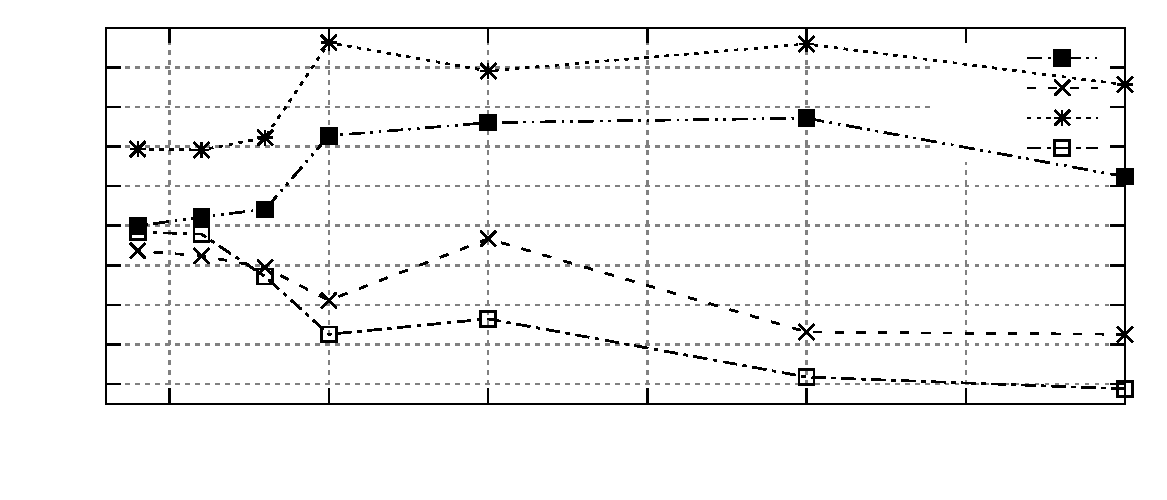
\includegraphics{StressToDiscreteness}}%
    \gplfronttext
  \end{picture}%
\endgroup

\caption{Зависимость средних напряжений в отсеках от величины КЭ}
\label{fig:stressToDiscreteness}
\end{figure}

На основании полученных данных и исходя из трудоемкости процесса расчета модели была определена оптимальная величина конечного элемента для дальнейшей работы над моделью, принятая равной $0,11\text{м}$. 
%Ниже приведены картины НДС в месте стыка крыла с фюзеляжем при различных размерах конечного элемента. 
